\documentclass[pdftex,11pt,a4paper]{article}
\usepackage[utf8]{inputenc}


\usepackage[hidelinks]{hyperref}
\usepackage[text={16cm,24cm},centering]{geometry}

\usepackage{paracol}
\usepackage{blindtext}
\usepackage{amsmath}


\setlength{\parskip}{1em}
%\usepackage[onehalfspacing]{setspace}

\renewcommand\thesection{\arabic{section}}
\renewcommand\thesubsection{\thesection.\arabic{subsection}}
\renewcommand\thesubsubsection{\thesubsection.\arabic{subsubsection}}

%\usepackage{natbib}
\usepackage{graphicx}
\usepackage{imakeidx}
\usepackage{changepage}   % for the adjustwidth environment
\makeindex[columns=3, title=Alphabetical Index, intoc]

\begin{document}
%\maketitle
%% Document settings
%{

\newcommand{\setlocalcolumnwidth}[1]{%
	%\let\oldratio\pcol@columnratioleft
	\setcolumnwidth{#1}%
}

\newcommand{\HRule}{\centering{\rule{1\linewidth}{1.5pt}}} % New command to make the lines in the title page

\newcommand{\decoRule}{\rule{.8\textwidth}{.4pt}} % New command for a rule to be used under figures

%}

\begin{titlepage}

\vspace{-20cm}
   \begin{center}

%      \setlength{\leftskip}{5mm}
\setlocalcolumnwidth{0.2\textwidth,0.6\textwidth,0.2\textwidth}
\begin{paracol}{3}
	
	\hspace{-1cm}
\includegraphics[scale = 0.2]{eie.jpg}
	\switchcolumn
	{\LARGE School of Electrical and Information Engineering}
	         {\large \\University of the Witwatersrand} 
	         {\small \\Johannesburg, South Africa}
	         \HRule \\[0.1cm]
	         \vspace{3cm}
	\switchcolumn
		
\includegraphics[scale = 0.23]{wits-orig.png}
\end{paracol}

\textbf{\Large DESIGN OF A ROBUST CODEC \\ \vspace{0.2cm} FOR A FADING}

\vspace{0.5cm}
         ELEN4011: DESIGN II
 
       \vspace{1.5cm}
 
       \textbf{Author:} Boikanyo Radiokana (1386807) \\
       \vspace{1.5cm}
       \textbf{Supervisor:} Prof. Fambarai Takawira
       \vspace{1cm}
       
       25 October 2019
       \vfill

\begin{adjustwidth}{5mm}{}
\textbf{Abstract:} To separate these two sections out we'll use the command which will automatically add in the amount of vertical space needed for the content to fill the page. Next we'll add in a line of text to specify what degree the thesis is being submitted for. The double backslash is used to create a new line. We'll then add more space before adding in the university logo specifying it's width as a fraction of the text width. Finally we'll add in some information about the university and the date.
\end{adjustwidth}

%\setlength{\rightskip}{-1cm}
       

       
 
   \end{center}
\end{titlepage}

\tableofcontents

\newpage
\section{Introduction}
Over the past years, the Telecommunications industry has seen a significant growth in demand for highly reliable wireless communication links that are capable of transmitting data at high rates. Unfortunately, like any other type of channel, a wireless channel has its own shortcomings. It is prone to noise, fading, reflection and shadowing \cite{22}. To combat these challenges, commonly used Forward Error Correction (FEC) techniques have been adopted in many applications to improve the reliability of data transmission. FEC enables data to be transmitted over long distances at low transmit power and at low Bit Error Rates, however, it requires an increase in channel bandwidth \cite{22}, \cite{18}.

To compensate for this, a widely used technology, MIMO architecture has been extensively explored and implemented \cite{18_1}, \cite{42}. It makes use of multiple transmit and receive antennas to improve the quality of digital communication systems. The key benefits of MIMO technology include an increase in channel capacity, high spectral efficiency as well as high data rates \cite{3}. MIMO systems have been found to have a linear increase in channel capacity with the minimum number of transmit and receive antennas \cite{42}.

In this paper, the design, analysis and simulation of a robust codec for a fading channel with MIMO architecture is presented. Section 2, 3 and 4 respectively present the design specifications, system model and the methodology adopted. Section 5, 6 and 7 details the simulation results, analysis and impacts of this type of technology on the society, the economy and the environment.




%%%%%%%%%%%%%%%%%%%%%%%%%%%%%%%%%%%%%%%%%%%%%%%%%%%%%%%%%%%%%%%%%%%%%%%%%%%%%%%
%
\section{Design Specifications}
The main objective of this project is to design a robust codec for a fading channel with an appropriate MIMO architecture that will combat the effects of fading. The following requirements and assumptions are taken into consideration when designing the codec. 

\subsection{Requirements and Success Criteria}
For the design to be deemed successful, the following requirements must be fullfilled:

\begin{itemize}
    \item The codec must achieve a spectral efficiency of at least $2bits/Hz$.
    \item The codec must be modelled for a Rayleigh fading channel.
    \item The data transmission of at least $10Mbits/sec$ must be achieved. 
\end{itemize}{}

\subsection{Assumptions}
The design is carried out with the following assumptions for simplification purposes:

\begin{itemize}
    \item Source encoding has already been implemented, therefore, the input data stream is already converted to binary format.
    \item Data encryption is not a primary component in this project, hence, it is optional.
    \item Channel State Information (CSI) is known at both the transmitter and receiver, therefore, channel estimation is not necessary.
    \item It is assumed that the relative distance between the transmitter and the receiver will mostly remain constant, thus the effects of Doppler shifts are negligible. 
\end{itemize}{}

\section{System Model}
A digital communication system  is mainly composed of three subsystems, namely: the transmitter, channel and receiver. Figure \ref{fig:1} below depicts the proposed codec design modelled from the aforementioned subsystems. In this section, a brief description of the system model is provided. The design is simulated in MATLAB R2018b.


\begin{figure}[h!]
    \centering
    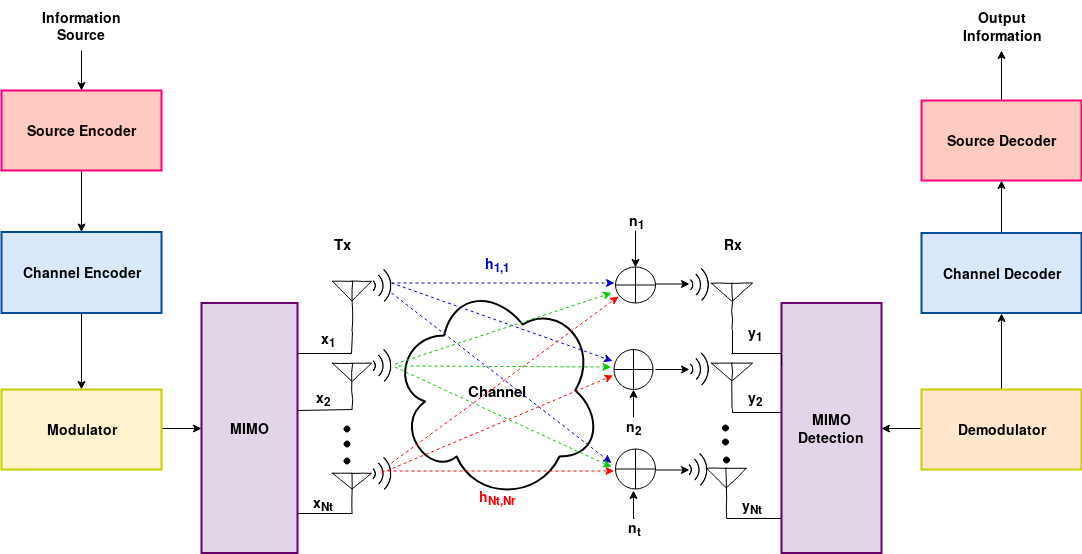
\includegraphics[width=\textwidth]{system5.png}
    \caption{System Model}
    \label{fig:1}
\end{figure}{}

The source of information can be a text, video or picture and this will require binary conversion before any signal processing can take place. This process of conversion includes reducing the bandwidth while containing significant components of the signal and this is performed by the source encoder and source decoder for reversal. As stated in section 2.2, it is assumed that the information source has already been conditioned to bit streams. This implies that source encoding and decoding will be disregarded in this design, thus the information source will be a randomly generated bit stream. 

The channel encoder is concerned with protecting the signal from channel noise, detecting and correcting errors present in the received signal through Forward Error Correction codes. This is achieved by introducing redundancy to the message at the encoder to ensure reliable transmission of information. Redundancy is exploited at the decoder to detect and correct any errors present in the message. 

Modulation involves impressing the codeword on a sinusoidal carrier and generating symbols which make it possible for efficient transmission over a noisy channel. Demodulation performed on the receiver end extracts the codeword from the symbols.

In a typical digital communication system, the symbols are transmitted through the channel after modulation. In this case, it goes through the MIMO architecture before being transmitted as seen in Figure \ref{fig:1}. There are types of MIMO techniques which arrange the symbols from a serial to parallel layout to allow symbols to be transmitted over multiple transmit and receive antennas. This reduces fading effects that the signal might encounter during transmission.

The channel is modelled in such a way that it introduces Rayleigh fading effects as well as Additive White Gaussian Noise.

\section{Design Methodology}
This section specifies and justifies the type of methods for each block that is illustrated in Figure \ref{fig:1}. Detailed mathematical computations for the respective blocks are provided.

\subsection{Forward Error Correction}
As mentioned earlier, wireless channels are prone to certain types of disturbances such as noise and fading. As a result, the received signal will contain errors. To protect the signal against errors, FEC codes are used. FEC codes add parity bits to the message in transit to introduce redundancy. The combination of the message and the parity bits are referred to as the \textit{Codeword}. FEC codes enable error detection and correction on the received codeword. Nevertheless, the codes have limitations to how many errors can be corrected. Error correction codes are classified into two categories, Convolutional Codes and Linear Block Codes. Turbo codes are a type of Convolutional Codes and BCH, RS and LDPC codes are types of Linear Block Codes. All the listed codes are capable of multiple error correction but differ in terms of complexity and implementation.

Turbo codes have been found to perform better than the listed codes because of its ability to provide exceptional coding gains and also perform close to the Shannon Limit \cite{18},\cite{18_7}. Turbo codes usually use large frames of more than 1000 bits since short frames introduce delays at the decoder \cite{chris}. The main disadvantage of using large frames is a highly complex decoder. Similarly, LDPC codes perform well, it is also known that the LDPC codes have a relatively complex decoder \cite{7online}.

A lot of research has been done to compare the performance between RS codes and BCH codes\cite{22}, \cite{9}, \cite{24}. It is found that RS codes are more suitable for concatenated codes and correcting burst errors. BCH codes on the other hand perform better than RS codes in Rayleigh Fading Channels with binary configurations \cite{22}. For this reason BCH codes are chosen for the design of the codec.

\subsubsection{BCH Encoder}
A BCH(\textit{n},\textit{k}) code with \textit{n} = 63, \textit{k} = 45 and a code rate \textit{r} = 0.714 is used since BCH codes with low redundancy and low error correction capability perform better \cite{14_7}. This is due to the fact that longer codewords require more bandwidth and have a high probability of errors. The BCH(63,45) code is capable of correcting a maximum of \textit{t} = 3 errors for a positive integer \textit{m}, where \(m\geq3\) and \(t<2^{m-1}\). The parameters of a BCH(\textit{n},\textit{k}) code are described by equations 1, 2 and 3 as follows:

\begin{equation}
	n = 2^{m}-1
\end{equation}
\begin{equation}
	n-k\leq mt
\end{equation}
\begin{equation}
	d_{min} \geq 2t -1
\end{equation}

wherein \textit{n} is the length of the codeword, \textit{k} is the length of the input message and \(d_{min}\) is the minimum distance. To encode the message \(m(x)\), the BCH encoder employs a generator polynomial \(g(x)\) defined by roots over the Galois Field GF($2^{m}$). Equation 4 describes \(g(x)\) for BCH(64,45).

\begin{equation} 
	g(x)= LCM\{\sigma_{1}(x),\sigma_{2}(x),... \sigma_{2t}(x)\}
\end{equation}

\begin{equation*} 
g(x)  =1 + x + x^2 + x^3 + x^6 + x^7 + x^9 + x^{15} + x^{16} + x^{17} + x^{18}
\end{equation*}

with \(\sigma_{i}(x)\) being the minimal polynomial. The remainder \(r(x)\) as depicted in Equation 5 is then calculated to find the parity check bits.

\begin{equation}
	r(x) = mod(m(x), g(x)) 
\end{equation}

Finally, the codeword \(c(x)\) is found using Equation 6 below:

\begin{equation}
	c(x) = r(x) + m(x)
\end{equation}

The BCH Encoder is the the first object that affects the data rate \textit{$R_{b}$} of $10Mbits/sec$ coming from the source. The resulting data rate after encoding is completed is presented by the equation below:

\begin{equation}
	R_{bfec} = \frac{10Mbits/sec}{r} = 14Mbits/sec
\end{equation}

wherein r is the code rate as described above.

\subsubsection{BCH Decoder}
To retrieve the original message from the received codeword, all the syndromes of the codeword are computed. If any of the syndromes are zero, it means there is no error in the received codeword hence no further action is needed, else the errors need to be located and corrected. This would then be followed by determining the error location polynomial using the syndromes by applying the Berlekamp-Massey Algorithm. Once the error location polynomial has been found, errors are located and corrected.

\subsection{Digital Modulation}
In a digital communication system, the binary or digital data has to be translated to an analogue waveform before transmission occurs. This translation is performed in digital modulation by impressing the message signal on a sinusoidal carrier waveform with a carrier frequency \text{$f_c$}. Modulation gives the message signal immunity to noise in a channel. It moves the spectrum of the baseband signal to frequencies close to that of the carrier frequency which is generally high frequencies in the M-GHz ranges. However, the translated baseband signal still has to adhere to the power constraints of the signal such that there is no interefernce between users within that spectrum \cite{book10}. The effect of noise immunity minimizes the Bit Error Rate (BER) while conserving the power and bandwidth. The resulting modulated signal is a sequence of sinusoids which can be expressed as complex signals also referred to as \textit{Symbols}. Modulation schemes are determined by which property of the carrier has been modified. These properties are the amplitude, frequency and phase of the carrier.

\subsubsection{Amplitude Phase Keying (ASK)}
In ASK Modulation the codeword is mapped to only the amplitude of the carrier by modifying it based on the state of the input codeword. ASK works in such a way that if the input is a 0 then the modulated signal will also be a 0, else if the input is a 1 then the modulated signal will be a sinusoid with amplitude \textit{A}. The advantage of using ASK is that it requires less bandwidth of \(W = 2f_b\) and also has a relatively simple demodulator \cite{61_}. One major flaw with using ASK is that it is highly susceptible to noise which means the transmitted signal will experience high attenuation.  ASK is mostly used in fibre optics communications and this design is focused on wireless systems, therefore it is not applicable. 



\subsubsection{Phase shift Keying (PSK)}
In PSK modulation only the phase of the carrier is changed. If the input is a 1 then the output of the modulator will be in-phase with the carrier, else, the output will be out of phase by $\pi$. PSK is bandwidth efficient because it occupies the same bandwidth as ASK and also offers high noise immunity \cite{61_}. In an M-ary PSK modulator, the unique patterns of bits are mapped to different carriers with different phases. Since PSK has a circular strcuture, all points are the same distance from the origin. Therefore, the higher the modulation order, the closer the constellation points are to each other. This modulation scheme has a tradeoff between increased bit rates (large M) and an increase in the probability of errors in  de-mapping the symbols due to a compact constellation structure \cite{unknownBook}. PSK is also known to have a complex demodulator. The applications of PSK include bluetooth technology, WLAN and radio frequency identification \cite{64}.

\subsubsection{Frequency Shift Keying (FSK)}
FSK only modifies the frequency of the carrier to represent the codeword. If a 1 is transmitted a different carrier frequency \(f_{c1}\) is used and if a 0 is transmitted \(f_{c2}\) is used. Even though FSK has high noise immunity and a moderate complex demodulator compared to PSK, it requires twice the bandwidth (
\(W = 4f_b\)) of PSK and ASK. Considering that bandwidth is a sacred commodity, FSK is not feasible. One major drawback with FSK is that it provides poor spectral efficiency \cite{smith}.

\subsubsection{Quadrature Amplitude Modulation (M-QAM)}
M-QAM modulation is one of the mostly used modulation schemes because of its ability to provide high spectral efficiencies, high transmission rates and energy efficiency \cite{65_10}, \cite{65_11}. For this reason it will be used in the design.

Quadrature Amplitude Modulation is a hybrid of ASK and PSK modulation schemes \cite{unknownBook}. The modulated signal is produced by initially applying a serial to 2-parallel word generator. The parallel sets of data will then be used to modulate the In-phase (I) and Quadrature (Q) components with the same carrier frequency and different amplitudes \cite{65}. Both these components are added to form the modulated signal \textit{s(t)} as illustrated in Figure 2.

\begin{figure}[h!]
	\centering
	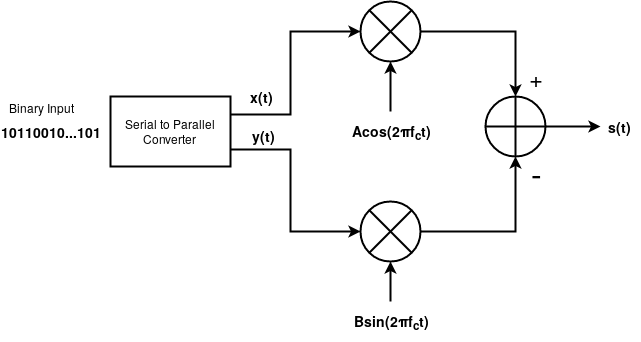
\includegraphics[scale=0.53]{QAM.png}
	\caption{QAM Modulator}
	\label{fig:1}
\end{figure}{}

The resulting modulated signal is defined in Equation 8 which can further be expressed as a complex symbol, Equation 9.

\begin{equation}
	s(t) = Acos(2\pi f_{ct}) - Bsin(2\pi f_{c}t)
\end{equation}
\begin{equation}
s = A - jB
\end{equation}

In an M-QAM modulation scheme there are M possible symbols which used to represent a codeword. Each symbol contains \(k = log_{2}M\) bits. Table 1 shows which M-QAM modulation orders will be investigated as well as the symbol rates. The symbol rate \(R_s\) is determined using Equation 10 below:

\begin{equation}
	R_s = \frac{R_b}{rlog_{2}M}
\end{equation}

wherein r is the code rate of the BCH encoder, \(R_b\) is the information source data rate and M is the modulation order.

\begin{table}[]
	\centering
	\caption{M-QAM Parameters}
	\label{1}
	\begin{tabular}{|c|l|l|l|}
		\hline
		\textbf{Modulation Order (M)}       & 16                       & 64                        & 128                    \\ \hline
		\textbf{Symbol Rate (Msymbols/sec)} & \multicolumn{1}{r|}{3.5} & \multicolumn{1}{c|}{2.33} & \multicolumn{1}{c|}{2} \\ \hline
	\end{tabular}
\end{table}
\subsubsection{M-QAM Demodulation}
To recover the original codeword, the M-QAM demodulator uses a coherent demodulator. The demodulator makes use of 2 cascaded mixers, lowpass filters and a symbol demapper \cite{B15}. Two carrier  signals are fed into the mixer and its outputs are sent to lowpass filters. The lowpass filter will attenuate the noise introduced during transmission. The symbol demapper will try to map the resulting symbol to one of the possible unique patterns of bits. The decision used to map the symbol is a Hard decision algorithm. In a Hard decision algorithm, the Hamming distance between the received codeword and all the possible patterns of bits are calculated. The pattern which yields the minimum hamming distance is chosen.

\subsection{Rayleigh Fading Channel}

\subsection{MIMO}


\subsubsection{STBC}
\subsubsection{Spartial Multiplexing}
\subsection{MIMO Receiver}


\section{Simulation Results}
\section{Critical Analysis}

\section{Future Recommendations}
\section{Impacts}

\section{Conclusion}
\newpage
\bibliographystyle{witseie}
\bibliography{references}

\end{document}
